\documentclass[border=10pt]{standalone}
\usepackage{tikz}
\usetikzlibrary{arrows.meta, positioning}

\begin{document}
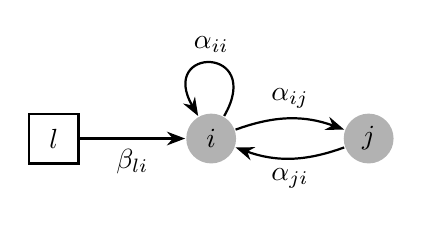
\begin{tikzpicture}[->, >=Stealth, thick, node distance=2cm]

  % Stili dei nodi
  \tikzstyle{state} = [circle, draw=none, fill=gray!60, minimum size=18pt, inner sep=2pt]
  \tikzstyle{input} = [rectangle, draw=black, fill=none, minimum size=18pt]

  % Nodi
  \node[input] (l) {$l$};
  \node[state, right of=l] (i) {$i$};
  \node[state, right of=i] (j) {$j$};

  % Frecce
  \draw[->] (l) -- (i) node[midway, below] {$\beta_{li}$};
  \draw[->, looseness=8, in=120, out=60] (i) to node[midway, above] {$\alpha_{ii}$} (i); % self loop
  \draw[->, bend left=20] (i) to node[midway, above] {$\alpha_{ij}$} (j);
  \draw[->, bend left=20] (j) to node[midway, below] {$\alpha_{ji}$} (i);

\end{tikzpicture}
\end{document}